\chapter{Introduction}\label{chapter:introduction}

\section{Project Overview}\label{sec:project-overview}

Large language models can answer scientific questions, act as tutors, and support decisions, but they can also state an incorrect answer in fluent and assertive language. Multi-agent debate addresses this by having several agents answer the same question and revise after reading each other's reasoning~\cite{du2024improving}. Chain-of-thought prompting exposes intermediate steps for the other agents to evaluate~\cite{wei2022chain}. The hard part is aggregating the agents' answers. Most systems use a vote in which every agent has equal weight and the most frequent answer wins~\cite{wang-etal-2024-rethinking-bounds,choi2025debate}. That rule treats repetition as evidence. Scientific inquiry does not. This report examines a trust-calibrated deliberation framework that gives each agent influence according to how well its claims match retrieved scientific evidence.

\section{Motivation}\label{sec:motivation}

Debate does not guarantee correctness. Agents can imitate one another or change position under social pressure even when one agent is right. In one study of three-agent debates, 25.5\% of the cases in which the agents disagreed had the correct answer in the minority, so majority voting discarded it~\cite{he2026minority}. Training models to be agreeable can also increase sycophancy and reduce accuracy~\cite{ibrahim2026training}. Majority voting is vulnerable because a confident majority can pressure a correct minority into switching, and the resulting unanimity hides the error. The risk is highest for scientific questions, where a user may trust a confident but unsupported answer. Existing methods address parts of the problem: iMAD predicts whether a debate is needed~\cite{fan2026imad}, DebUnc weights agents by self-reported uncertainty~\cite{yoffe-etal-2025-debunc}, and Mixture-of-Agents combines outputs with static aggregation~\cite{wang2025mixture}. None of these methods ties an agent's influence to whether its claims continue to match external evidence during the debate. This study adds that connection.

\section{Objectives}\label{sec:objectives}

The objective is to test whether evidence-weighted trust reduces sycophantic collapse relative to majority voting in multi-agent LLM debate. The work has two parts. First, it characterizes the failure: a confident majority can pressure a correct minority into changing its answer~\cite{he2026minority,pitre-etal-2025-consensagent}. Second, it designs and implements a bounded trust mechanism. Trust rises when retrieved evidence supports an agent's claims and falls when it contradicts them. The trust vector is projected onto a simplex with a floor after every update, so no agent disappears and no agent dominates. The final answer is a trust-weighted plurality, not a head count. The evaluation compares this mechanism with majority voting and other debate and aggregation methods~\cite{choi2025debate,wang-etal-2024-rethinking-bounds}; the planned endpoints are final-answer accuracy, correct-minority retention, collapse under pressure, appropriate revision, and trust calibration.

\section{Methodology}\label{sec:methodology}

This study uses an experimental methodology. We first build a vanilla multi-agent debate baseline. Several diverse language-model agents answer the same science question and revise their positions after reading each other's reasoning over three rounds~\cite{du2024improving}. The baseline aggregates the final positions by majority vote, which exposes the failure modes that the trust mechanism is designed to address~\cite{choi2025debate}. We then decompose each agent's response into claims and check each claim against scientific literature retrieved from external sources~\cite{karpukhin2020dense}. A verifier assigns each claim to supported, contradicted, or unverifiable~\cite{kushwaha2026agentbased}. Support and contradiction update the agent's trust; unverifiable claims do not move it. Unlike DebUnc, the signal here is external evidence, not self-reported confidence~\cite{yoffe-etal-2025-debunc}. The trust vector is bounded by the simplex projection described in Chapter~3, and the final answer is a trust-weighted plurality. The models are used inference-only, without fine-tuning. The framework has been exercised end to end on a ten-question GPQA slice (Gate~0), which validates serving, orchestration, and parsing. The comparative evaluation on GPQA-Main and MMLU-Pro is planned; no comparative result is reported here.

\section{Project Outcome}\label{sec:project-outcome}

The project produces a reproducible framework for trust-calibrated scientific deliberation. Agent influence is updated from retrieved evidence while the debate runs, and the final answer comes from evidence-weighted trust rather than a majority count. The project also produces an evaluation protocol. The protocol defines final-answer accuracy, correct-minority retention, collapse under pressure, appropriate revision, and trust calibration, and it specifies a pre-registered matrix. It is designed to detect sycophantic collapse~\cite{pitre-etal-2025-consensagent} and to track whether correct minority answers survive~\cite{he2026minority}. A wrong answer can still win. The method records which agents the evidence supported and which it contradicted, so the decision is auditable.

\section{Organization of the Report}\label{sec:organization-of-the-report}

Chapter~2 covers multi-agent debate and sycophancy and defines the gap this study addresses. Chapter~3 records the requirements, the methodology, the system design, and the project plan. Chapter~4 describes the implementation environment, the pipeline, the P0 hardening changes, and the validation evidence available at mid-project. Chapter~5 covers standards, design constraints, sustainability, and the complex engineering analysis. Chapter~6 closes with a summary, the limits of the evidence, and directions for future work.

\begin{figure}[ht]
    \centering
    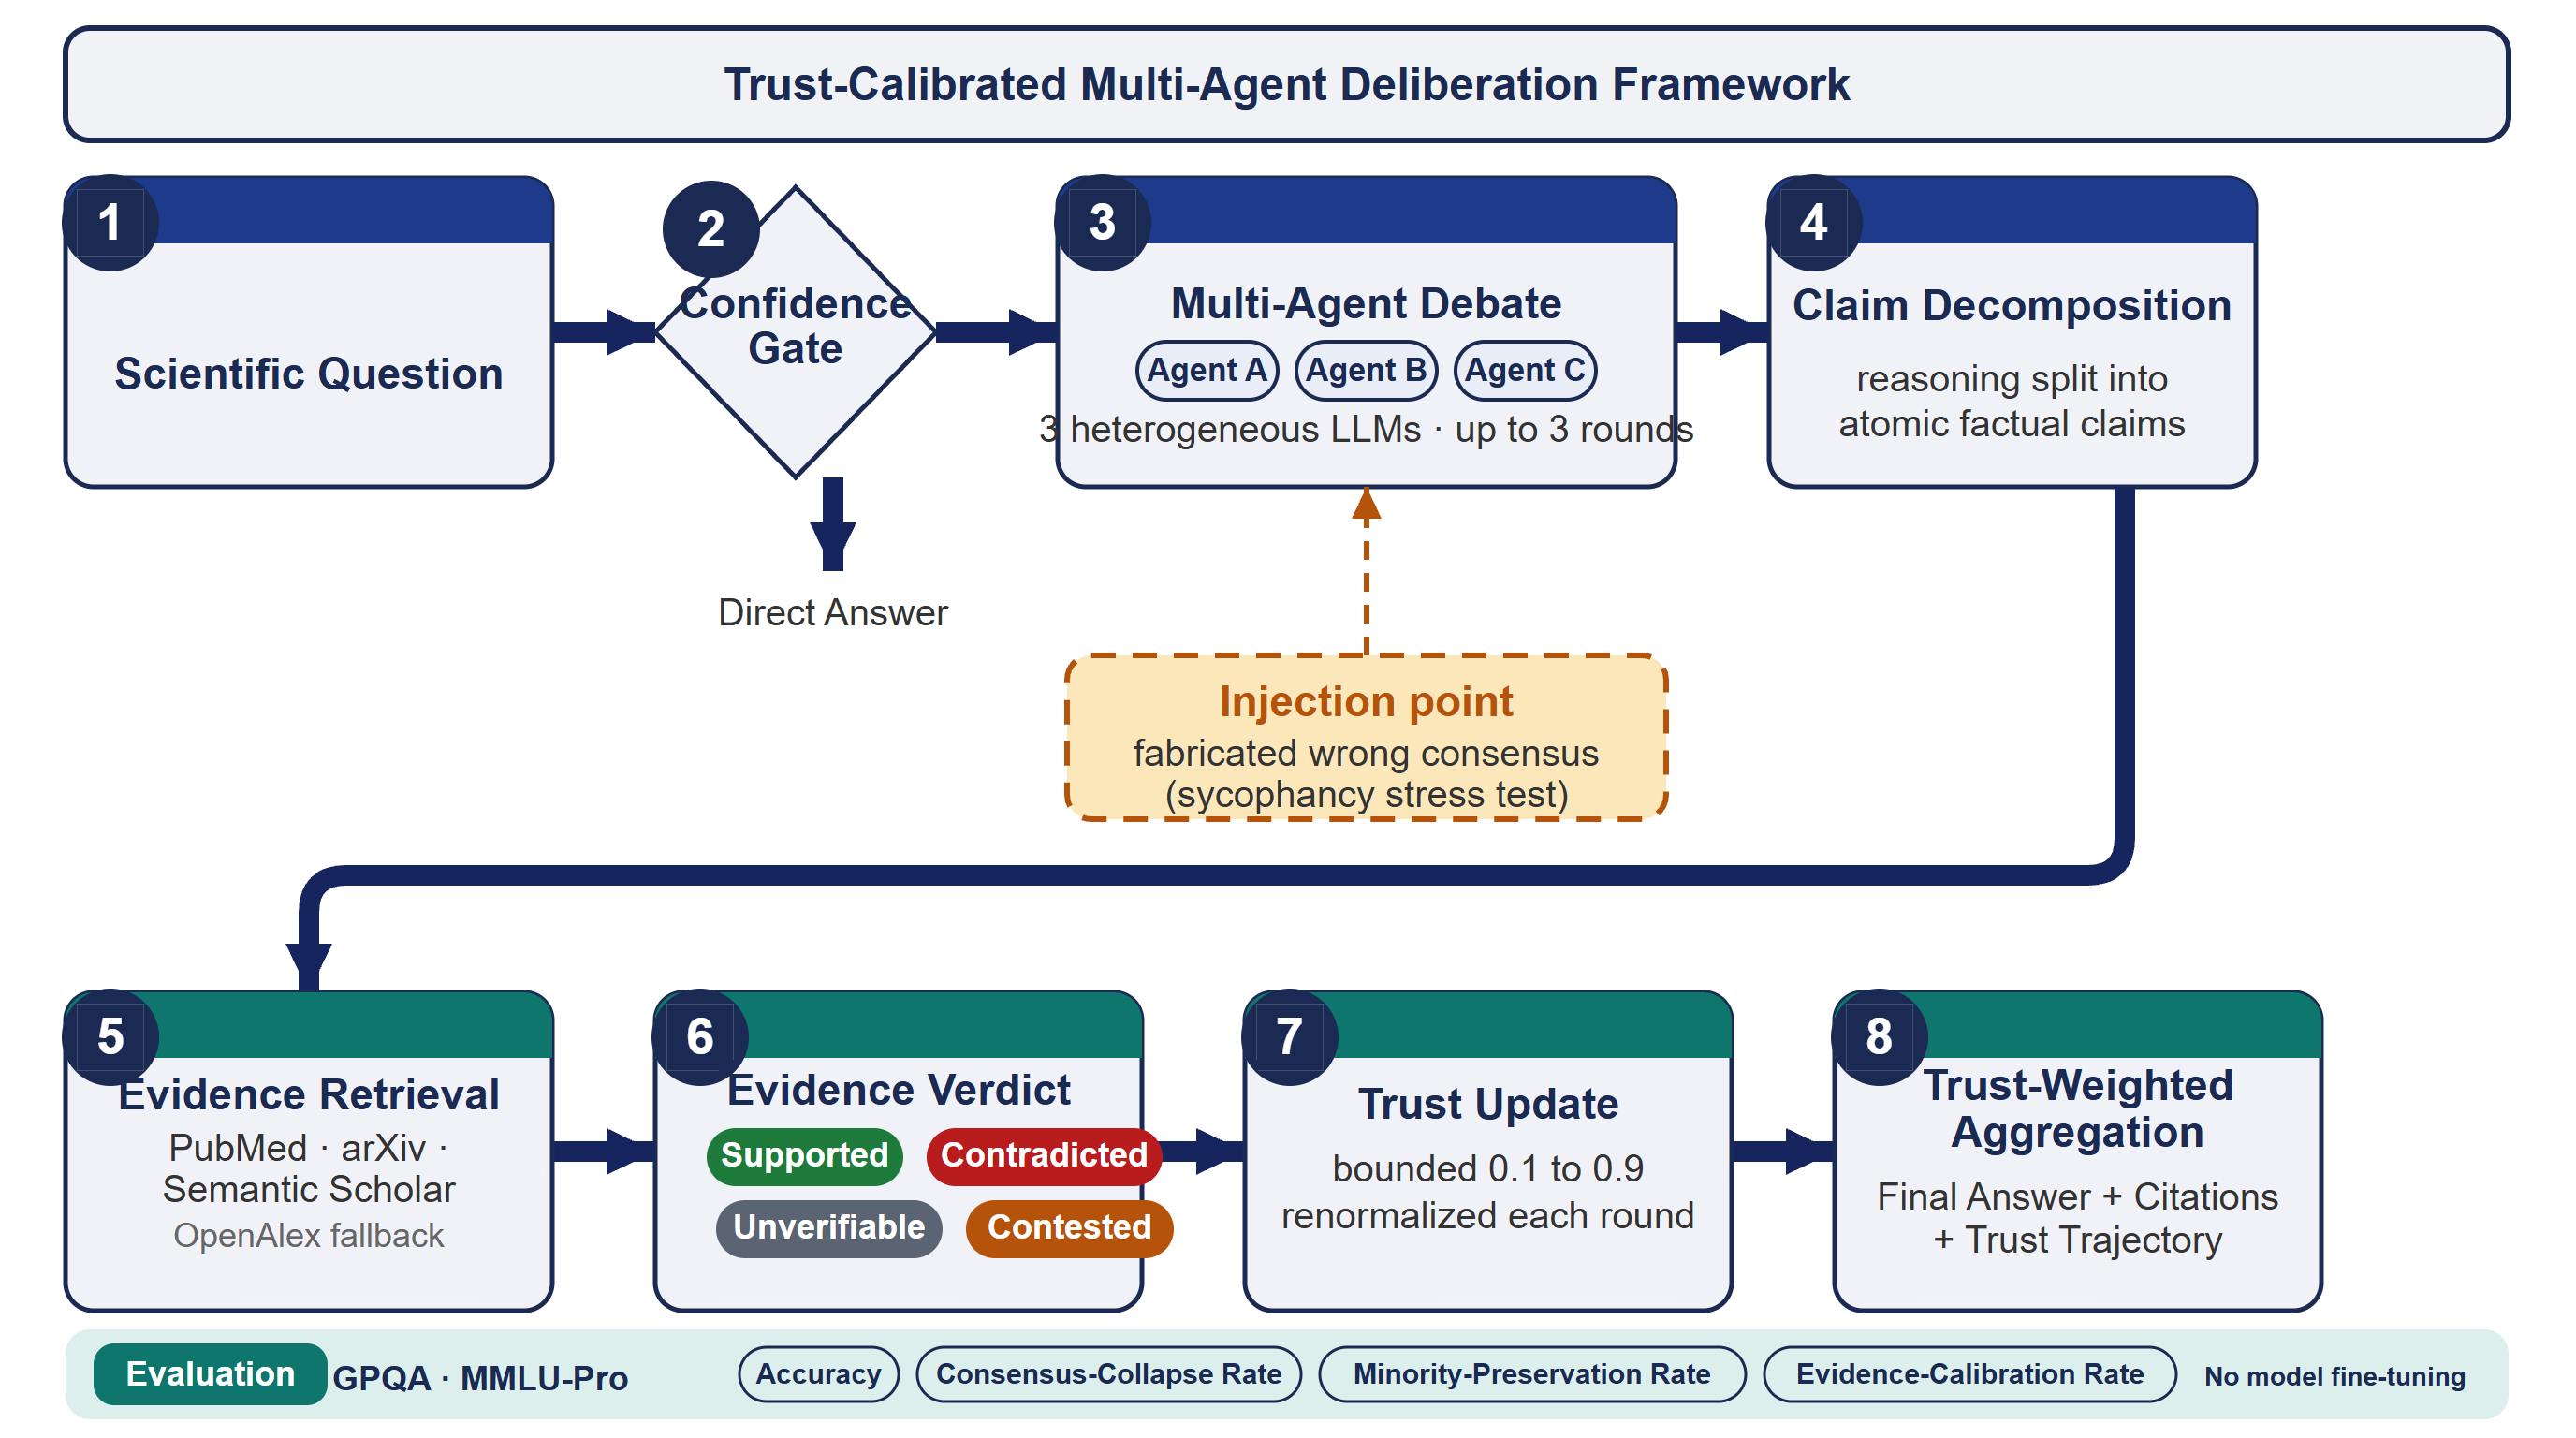
\includegraphics[width=\textwidth]{fig-pipeline.png}
    \caption{End-to-end flow: seeded option rendering, three-round debate, claim decomposition, claim-domain retrieval, verifier labels, logit accumulation with one softmax and a simplex projection, one-shot injection during revision, and trust-weighted aggregation using the final trust vector.}
    \label{fig:methodology-flow}
\end{figure}
